%% Copyright (C) 2009-2010, Gostai S.A.S.
%%
%% This software is provided "as is" without warranty of any kind,
%% either expressed or implied, including but not limited to the
%% implied warranties of fitness for a particular purpose.
%%
%% See the LICENSE file for more information.

\newcommand{\refFacet}[2][]%
  {\hyperref[sec:interface:#2]{\lstinline|#2|#1 (\autoref*{sec:interface:#2})}}

\newcommand{\interface}[2][]{%
  \ifthenelse{\equal{#1}{}}{%
    \subsection{#2\index{#2@\lstinline{#2}}}%
  }{%
    \subsection{#2 (subclass of #1)\index{#2@\lstinline{#2}}}%
  }%
  \defObject{Interface.#2}%
  \label{sec:interface:#2}
}

\newcommand{\gsrapi}{Gostai Standard Robotics API\xspace}
\chapter{Gostai Standard Robotics API}
\label{sec:naming}


This section aims at clarifying the naming conventions in \urbi
Engines for standard hardware/software devices and components
implemented as UObject and the corresponding methods/attributes/events
to access them. The list of available hardware types and software
component is increasing and this document will be updated
accordingly. Please contact us directly, should you be working on a
component not described or closely related to one described here:

\begin{center}
  \email{standard@gostai.com}
\end{center}

Any implementation of an \urbi server must comply with the latest
version of this standard to get the ``\urbi Ready'' certification from
Gostai S.A.S.

Gostai S.A.S. is currently the only authority which has the ability to
deliver an ``\urbi Ready'' certification.

``\urbi Ready'' and the associated logo are trademarks of Gostai
S.A.S. and should not be used or displayed in any way without an
explicit written agreement from Gostai.

\section{The Structure Tree}

The robot will be described as a set of \dfn[component]{components} organized
in a hierarchical structure called the \dfn{structure tree}. The
relationship between a component and a sub-component in the tree is a
`part-of' inclusion relationship. From the point of view of \urbi,
each component in the tree is an object, and it contains attributes
pointing to its sub-components. Here is an example illustrating a part
of a hierarchy that could be found with a wheeled robot with a gripper:

\begin{center}
  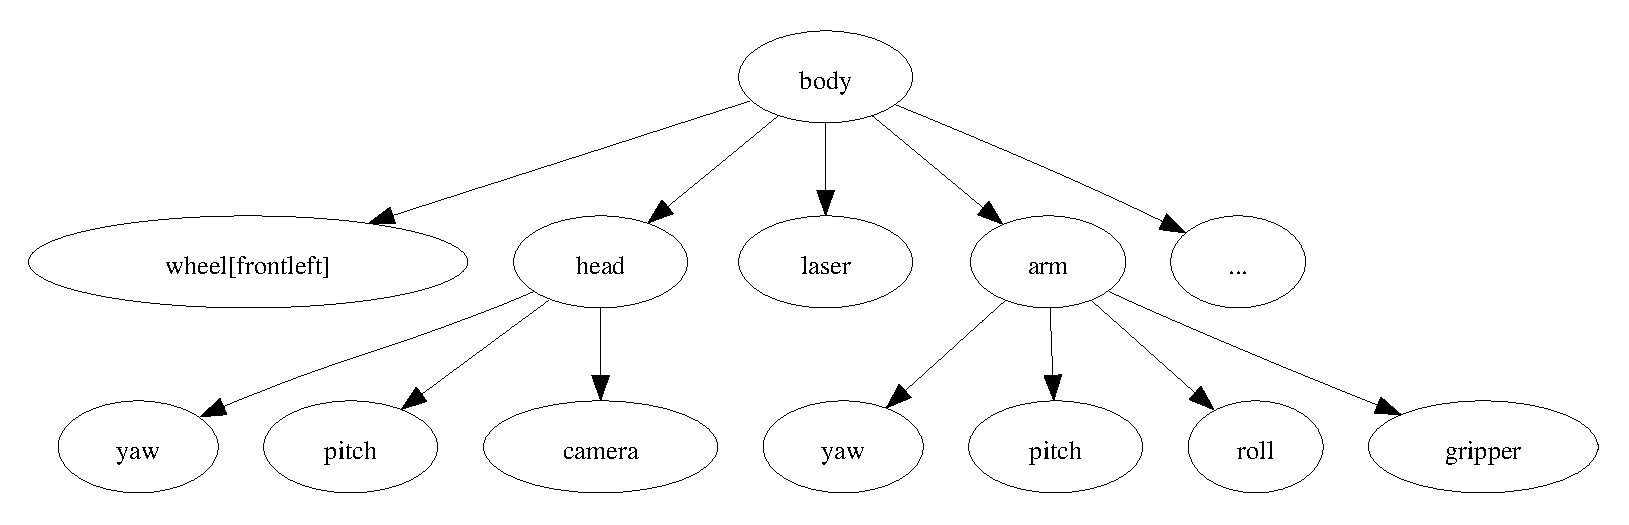
\includegraphics[width=.8\linewidth]{img/structure-tree-wheeled}
\end{center}

And here is another example for an humanoid robot:

\begin{center}
  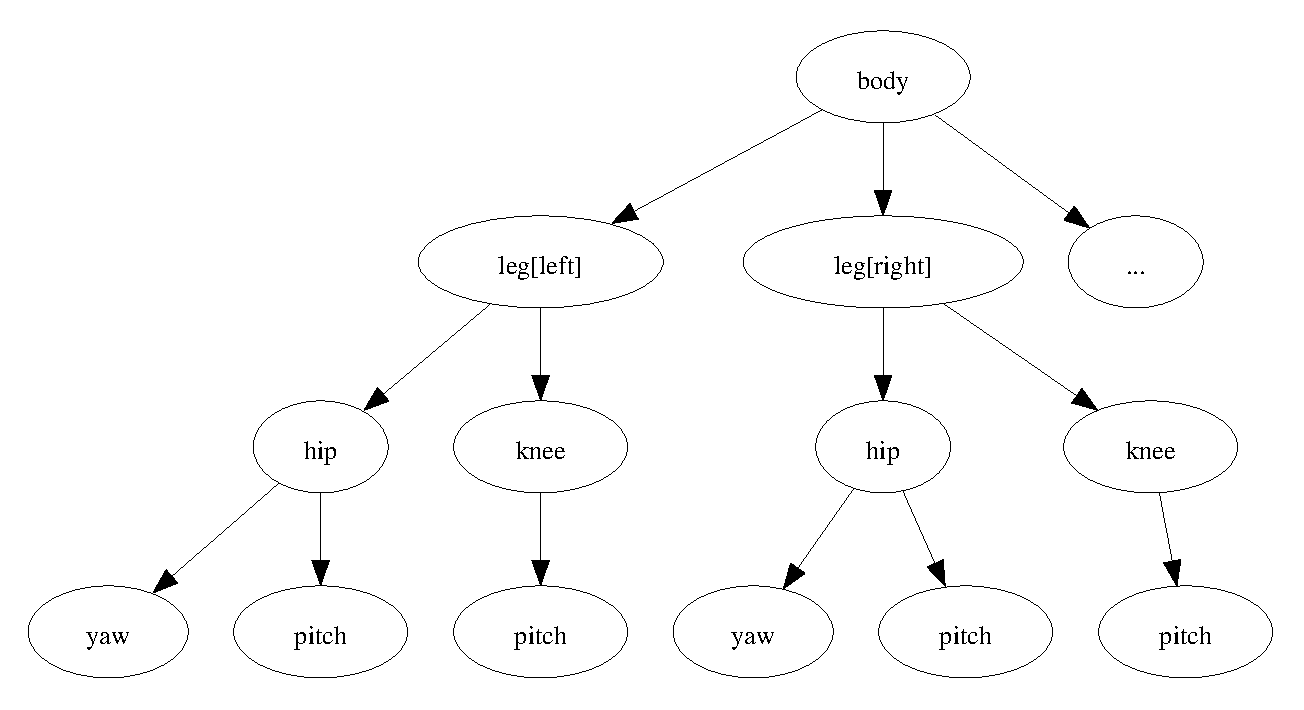
\includegraphics[width=.8\linewidth]{img/structure-tree-humanoid}
\end{center}

The leaves of the tree are called \textit{devices}, and they usually
match physical devices in the robot: motors, sensors, lights, camera,
etc. Inside \urbi, the various objects corresponding to the tree
components are accessed by following the path of objects inclusions,
like in the example below (shortcuts will be described later):

\begin{urbiunchecked}
body.leg[right].hip.tilt;
body.arm.grip;
body.laser;
// ...
\end{urbiunchecked}


The structure tree should not be mistaken for a representation of the
kinematics chain of the robot. The kinematics chain is built from a
subset of the devices corresponding to motor devices, and it
represents spatial connections between them. Except for these motor
devices, the structure tree components do not have a direct
counterpart in the kinematics chain, or, if they do, it is as a subset
of the kinematics chain (for example, \code{leg[right]} is a subset of the
whole kinematics chain).


The goal of this standard is to provide guidelines on how to define
the components and the structure tree, knowing the kinematics chain of
the robot.

\section{Frame of Reference}

In many cases, it will be necessary to refer to an absolute frame of
reference attached to the robot body. To avoid ambiguities, the
standard frame of reference will have the following definition:

\begin{center}
  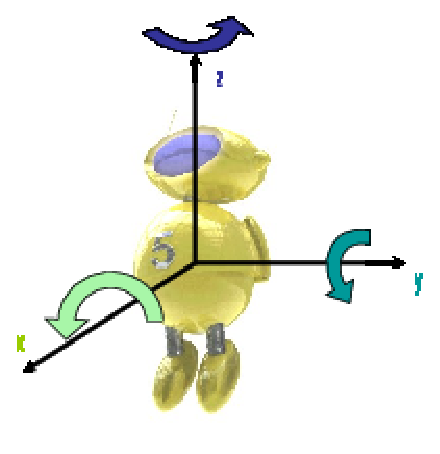
\includegraphics{img/reference-frame}
\end{center}

\begin{description}
\item[Origin] the center of mass of the robot
\item[X axis] oriented towards the front of the robot. If there is a
  camera, the front is defined by the default direction of the camera,
  otherwise the front will be seen as the natural frontal orientation
  for a mobile robot (the direction of ``forward'' movement). If the
  robot is not naturally oriented, the X axis will be chosen to match
  the main axis of symmetry of the robot body and it will be oriented
  towards the smallest side, typically the top of a cone for
  example. In case of a perfectly symmetrical body, the X axis can be
  chosen arbitrarily but a clear mark should be made visible on the
  robot body to indicate it.
\item[Z axis] oriented in the opposite direction from the gravity. If
  there is no gravity or natural up/down orientation in the
  environment or normal operation mode of the robot, the Z axis should
  be chosen in the direction of the main axis of symmetry in the
  orthogonal plane defined by the X axis, oriented towards the
  smallest side. In case of a perfectly symmetrical plane, the Z axis
  can be chosen arbitrarily but a clear mark should be made visible on
  the robot body to indicate it.
\item[Y axis] oriented to make a right-handed coordinate system.
\end{description}


The axes are oriented in a counter-clockwise direction, as depicted in
the illustration above.

\section{Component naming}

Each component A, which is a sub-component of component B has a name, distinct
from the name of all the other components at the same level.
This name is a generic designation of what A represents, such as ``leg''
,``head'', or ``finger''.

Using the correct name for each component is a critical part of this standard.
No formal rule can be given to find this name for any possible robot
configuration. However, this document includes a table covering many different
possible cases. We recommend that robot manufacturers pick from this table
the name that fits the most the description of their component.

\section{Localization}
When two identical components A1 and A2, such as the two legs of an humanoid
robots, are present in the same sub-component B, an extra node is inserted in
the hierarchy to differentiate them. This node is of the \code{Localizer} type,
and provides a \code{[]} operator, taking a \code{Localization} argument, used
to access each of the identical sub-components.
The \usdk provides an implementation for the \code{Localizer} and
\code{Localization} classes.
When possible, localization should be simple geometrical qualifier like
\textit{right}/\textit{center}/\textit{left},
\textit{front}/\textit{middle}/\textit{back} or
\textit{up}/\textit{in-between}/\textit{down}.
Note that ``right'' or ``front'' are
understood here from the point of view of a man standing and looking
in the direction of the X-axis of the robot, and \textit{up/pown}
matches the Z-axis, as depicted in the figure below:

\begin{center}
  
\includegraphics[width=.5\linewidth]{img/cube}
\end{center}

Several geometric qualifiers can be used at the same time to further
refine the position. In this case, multiple Localizer nodes are used.
As a convention, height information (U/I/D) comes first,
followed by depth information (F/M/H), and then side information (R/C/L).

\begin{urbiunchecked}
// Front-left wheel of a four-wheeled robot:
robot.body.wheel[front][left];
// Front laser of a robot equipped with multiple sonars:
robot.body.laser[front];
// Left camera from a robot with a stereo camera at the end of an arm:
robot.body.arm.camera[left];
// Top-left LED of the left eye.
robot.body.head.eye[left].led[up][left].val = 1;
// Touch sensor at the end of the front-left leg of a four-legged robot:
robot.body.leg[front][left].foot.touch;
\end{urbiunchecked}

You can further qualify a side+depth localization with an additional
F/B side information. This can be used in the typical layout below:

\begin{center}
  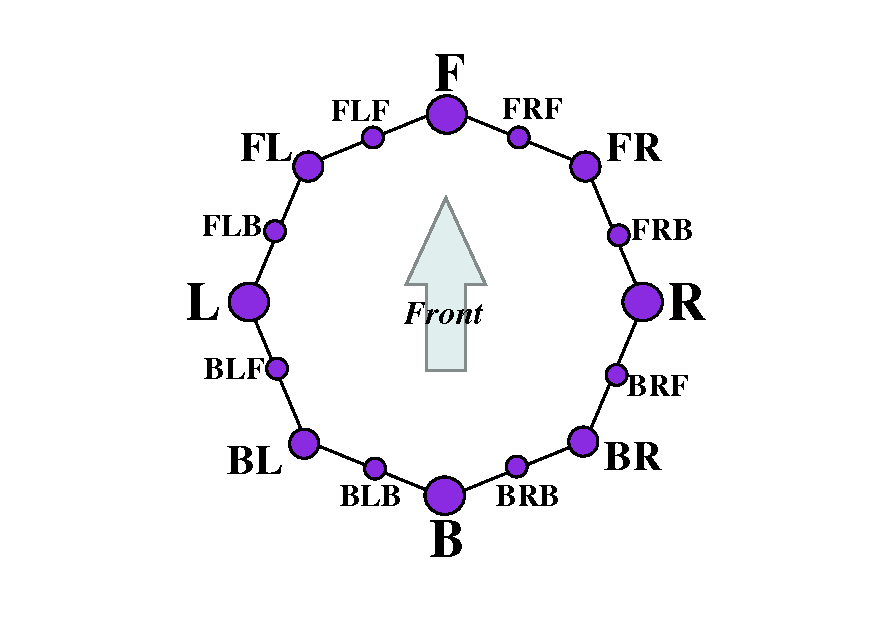
\includegraphics{img/localizer-multidim}
\end{center}

This dual positioning using side+depth can also be used to combine
side+height or height+depth information.

Layouts with a sequence of three or more identical components can use numbers
as their Localization, starting from 0.  The smaller the number, the closer to
the front, up, or left. For instance, an insectoid robot with 3 legs on each
side will use
\code{robot.body.leg[left][0]} to address the frontleft leg.

Layouts with identical components arranged in a circle can also use numeric
localization. The component with index 0 should be the uppermost, or front-most
if non applicable. Index should increase counterclockwise.

Some components like spines or tails are highly articulated with a set
of identical sub-components. When talking about these sub-components,
the above localization should be replaced by an array with a numbering
starting at 0. The smaller the number, the closer the sub-component is
to the robot main body. For surface-like sub-components, like skin
touch sensors, the array can be two dimensional.


Other possible localization for sensors are the X, Y and Z axis
themselves, like for example for an accelerometer or a gyro sensor,
available in each of the three directions.

\begin{urbiunchecked}
robot.body.accel[x]; // accelerometer in the x direction
\end{urbiunchecked}


Examples of component names including localization:

\begin{urbiunchecked}
leg[right], leg[left];
finger[right], finger[center], finger[left];      // three-finger hand
joint[0], joint[1] ... joint[5] // from tail
touch[478][124]                 // from skin
accel[x], accel[y], accel[z];         // typical accelerometer
gyro[x], gyro[y], gyro[z];            // typical gyro sensor
\end{urbiunchecked}

\section{Interface}
\label{sec:interface}

An ``interface'' describes some aspects of a type of device, by specifying the
slots and methods that implementations must provide. Each child node of
the component hierarchy should implement at least one interface.

For example, for a joint, we can have a ``Swivel'' interface, used to define
patella joints. For the robot body itself, we have a ``Mobile'' interface
describing mobile robots, which includes some standard way of
requesting a move forward, a turn, etc.

In short, interfaces are standard Urbi objects that components can inherit
from to declare that they have some functionalities.

The following pages describe a few of the most standard interfaces. Each
device in the component hierarchy which falls within the category of an
interface should implement it.

Each interface defines slots, which can be functions, events or plain data.
Some of those slots are optional: they are grayed and put around square
brackets in the following table.

\interface{Identity}

Contains information about the robot identity.

\begin{urbiscriptapi}
\item[type]%
  This describes the robot category among: humanoid, four-legged, wheeled,
  industrial arm. It gives a general idea of the robot family, but does not
  replace a more systematic probe of available services by investigating the
  list of attributes of the object.

\item[name]%
  Name of the robot.

\item[model] Model of the robot.

\item[serial] Serial number (if available).
\end{urbiscriptapi}


\interface{Network}

Contains information about the network identification of the robot.

\begin{urbiscriptapi}
\item[IP] IP address of the robot.
\end{urbiscriptapi}

\interface{Motor}

This interface is used to describe a generic motor controller.

\begin{urbiscriptapi}
\item[val] This slot is a generic pointer to a more specific slot describing
  the motor position, like \code{position} or \code{angle}, depending on the
  type of motor. It is mandatory in the Urbi Ready standard as a universal
  proxy to control an actuator. The more specific slot is described in a
  subclass of \code{Motor}.
\item[PGain?] Controls the P gain of the PID controller.
\item[IGain?] Controls the I gain of the PID controller.
\item[DGain?] Controls the D gain of the PID controller.
\end{urbiscriptapi}

\interface[Motor]{LinearMotor}


This interface is used to describe a linear motor controller.

A wheel can fall in this category, if the reported position is the distance
traveled by a point at the surface of the wheel.

\begin{urbiscriptapi}
\item[position] Position of the motor in meters.  Pointed to by the
  \code{val} slot.

\item[force] Intensity of the measured or estimated force applied on a
  linear motor.
\end{urbiscriptapi}

\interface[Motor]{LinearSpeedMotor}

Motor similar to \code{LinearMotor}, but controlled by its translation speed.

\begin{urbiscriptapi}
\item[speed] Translation speed in meters per second. Pointed to by the
  \code{val} slot.
\end{urbiscriptapi}


\interface[Motor]{RotationalMotor}


This interface is used to describe a position-controlled rotational motor
controller.

\begin{urbiscriptapi}
\item[angle] Angle of the motor in radian, modulo $2\pi$. Pointed to by the
  \code{val} slot.

\item[turn] Absolute angular position of the motor, expressed in number of
  turns.

\item[torque] Intensity of the measured or estimated torque applied on the
  motor.
\end{urbiscriptapi}

\interface[Motor]{RotationalSpeedMotor}

Interface describing a motor similar to \code{RotationalMotor} controlled
by its rotation speed.

\begin{urbiscriptapi}
\item[speed] Rotation speed in radians per second.
\end{urbiscriptapi}

\interface{Sensor}

This interface is used to describe a generic sensor.

\begin{urbiscriptapi}
\item[val] This slot is a generic pointer to a more specific slot describing
  the sensor value, like \code{distance} or \code{temperature}, depending on
  the type of sensor. It is mandatory in the Urbi Ready standard as a
  universal proxy to read a sensor. The more specific slot is described in a
  subclass of \code{Sensor}.
\end{urbiscriptapi}


\interface[Sensor]{DistanceSensor}

This interface is used to describe a distance sensor (infrared, laser,
ultrasonic...).

\begin{urbiscriptapi}
\item[distance] Measured distance expressed in meters.  Pointed to by the
  \code{val} slot.
\end{urbiscriptapi}


\interface[Sensor]{TouchSensor}

This interface is used to describe a touch pressure sensor (contact,
induction,...).

\begin{urbiscriptapi}
\item[pressure] Intensity of the pressure put on the touch sensor. Can be
  0/1 for simple buttons or expressed in Pascal units. Pointed to by the
  \code{val} slot.
\end{urbiscriptapi}


\interface[Sensor]{AccelerationSensor}

This interface is used to describe an accelerometer.

\begin{urbiscriptapi}
\item[acceleration] Acceleration expressed in $m/s^2$.  Pointed to by the
  \code{val} slot.
\end{urbiscriptapi}

\interface[Sensor]{GyroSensor}
This interface is used to describe an gyrometer.

\begin{urbiscriptapi}
\item[speed] Rotational speed in $\mathrm{rad}/s$.  Pointed to by the
  \code{val} slot.
\end{urbiscriptapi}

\interface[Sensor]{TemperatureSensor}
This interface is used to describe a temperature sensor.

\begin{urbiscriptapi}
\item[temperature] Measured temperature in Celsius degrees.  Pointed to by
  the \code{val} slot.
\end{urbiscriptapi}

\interface[Sensor]{Laser}
Interface for a scanning laser rangefinder, or other similar technologies.

\begin{urbiscriptapi}
\item[val] Last scan result. Can be either a list of ufloat, or a binary
  containing a packed array of doubles.

\item[angleMin] Start scan angle in radians, relative to the front of the
  device.

\item[angleMax] End scan angle in radians, relative to the front of the
  device.

\item[resolution] Angular resolution of the scan, in radians.

\item[distanceMin] Minimum measurable distance.

\item[distanceMax] Maximum measurable distance.

\item[rate?] Number of scans per second.
\end{urbiscriptapi}

Depending on the implementation, some of the parameters can be read-only, or
can only accept a few possible values. In that case it is up to the implementer
to select the closest possible value to what the user entered. It is the
responsibility of the user to read the parameter after setting it to check
what value will actually be used by the implementation.


\interface{Mobile}

Mobile robots all share this generic interface to provide high order
level motion control capabilities.

\subsubsection{Blocking API}

The following set of functions will block until associated movement is finished.
If a function of this set is called while an other is already running, the
first call will be cancelled: the movement will be interrupted and the
call will return.

Many of the functions below take a position argument. This position is expressed
as a subset of the six values x, y, z, rho, theta, phi.

\begin{urbiscriptapi}
\item[go](<x>) Move approximately \var{x} meters forward (along the X axis) if
\var{x} is positive, backward otherwise.

\item[turn](<theta>) Turn left (in the direction going from the positive X axis
to the positive Y axis) approximately \var{theta} radians.  \var{theta} can be a
  positive or negative value.

\item[goTo](<position>) Try to reach the given coordinates in the robot
frame of reference.

\item[gotoChargingStation]() Try to reach the charging station. If the feature
is not available, return immediately.

\item[gotoAbsolute](<position>) Try to reach given coordinates in an
absolute frame of reference. This frame of reference is maintained using the
robot odometry, or any other localisation system available.

\item[position] The current robot position in the absolute frame of reference.

\item[stop]() Stop current movement.

\item[setAbsolutePosition](<position>) Force absolute position to the given
value.
\end{urbiscriptapi}

\subsubsection{Speed-control API}

In addition to the previous functions, one can directly set the target movement
speed in all linear/angular directions using the 6 scalar variables xSpeed,
ySpeed, zSpeed, yawSpeed, pitchSpeed, rollSpeed, or the variable speed which
contains a list.
Writting to one of those slots will abort any function in the blocking API.

Implementations should provide default reasonable values for speed in the slots
defaultXSpeed, defaultYSpeed, defaultZSpeed, defaultYawSpeed, defaultPitchSpeed
and defaultRollSpeed.

\subsubsection{Safety}

\begin{urbiscriptapi}

\item{watchdogInterval} If non-zero, duration after which the robot will stop
if no order was received. Once activated, one has to write to
\lstinline|watchdog|, to one of the speed variables or call one of the
blocking API functions every \lstinline|watchdogInterval| at most, or the
stop() function will be called.
\item{watchdog} Writing any value to \lstinline|watchdog| will reset the
watchdog timer.

\end{urbiscriptapi}

\subsubsection{State}

\begin{urbiscriptapi}
\item[moving] True if the robot is currently moving for any reason, false
otherwise.
\item[aborted?] Emited each time a function in the blocking API is aborted
because it was preempted by an other movement.
\item[unreachable?] Emited when a function in the blocking API is aborted
because the target cannot be reached.
\item[finished?] Emited each time a function in the blocking API finished
normaly.

\end{urbiscriptapi}

\interface{Tracker}

Camera-equipped robots can sometimes move the orientation of the field
of view horizontally and vertically, which is a very important feature
for many applications. In that case, this interface abstracts how such
motion can be achieved, whether it is done with a pan/tilt camera or
with whole body motion or a combination of both.

\begin{urbiscriptapi}
\item[yaw] Rotational articulation around the Z axis in the robot, expressed
  in radians.
\item[pitch] Rotational articulation around the Y axis in the robot,
  expressed in radians.
\end{urbiscriptapi}

\interface{VideoIn}

The VideoIn interface groups every information relative to cameras or any
image sensor.

\begin{urbiscriptapi}
\item[val] Image represented as a \code{Binary} value.
\item[xfov] The x field of view of the camera expressed in radians.
\item[yfov] The y field of view of the camera expressed in radians.

\item[height] Height of the image in the current resolution, expressed in
  pixels.

\item[width] Width of the image in the current resolution, expressed in
  pixels

\item[format?]
    Format of the image, expressed as an integer in the enum
    urbi::UImageFormat.  See below for more information.

\item[exposure?] Exposure duration, expressed in seconds. 0 if non
  applicable.

\item[wb?]  White balance (expressed with an integer value depending on the
  camera documentation). 0 if non applicable.

\item[gain?]  Camera gain amplification (expressed as a coefficient between
  0 and infinity). 1 if non applicable.

\item[resolution?]  Image resolution, expressed as an integer. 0 corresponds
  to the maximal resolution of the camera. Successive values correspond to
  all the supported image sizes in decreasing order.  Once modified, the
  effective resolution in X/Y can be checked with the width and height
  slots.

\item[quality?]  If the image is in the jpeg format, this slot sets the
  compression quality, from 0 (best compression, worst quality) to 100 (best
  quality, bigger image).
\end{urbiscriptapi}

The image sensor is expected to use the cheapest way in term of CPU and/or
energy consumption to produce images of the requested format.
Implementations linked to a physical image sensor do not have to implement
all the possible formats. In this case, the format closest to what was
requested must be used.
A generic image conversion object will be provided. In order to avoid
duplicate image conversions when multiple unrelated behaviors need the same
format, it is recommended that this object be instantiated in a slot of the
VideoIn object named after the format it converts to:
\begin{urbiunchecked}
if (!robot.body.head.camera.hasSlot("jpeg"))
{
  var robot.body.head.camera.jpeg =
    ImageConversion.new(robot.body.head.camera.getSlot("val"));
  robot.body.head.camera.jpeg.format = 3;
}
\end{urbiunchecked}

\interface{AudioOut}
The AudioOut interface groups every information relative to speakers.

\begin{urbiscriptapi}
\item[val] The speaker value, expressed as a binary, in the format given by
  the binary header during the assignment.

  Speakers are write-only devices, so there is not much sense in reading the
  content of this attribute. At best, it returns the remaining sound to be
  played if it is not over yet, but this is not a requirement.


\item[remain] The amount of time remaining to play in the speaker sound
  buffer (expressed in \textit{ms} as a default unit).


\item[playing] This is a Boolean value which is true when there is a sound
  currently playing (the buffer is not empty)%

\item[volume?] Volume of the play back, in decibels.
\end{urbiscriptapi}



\interface{AudioIn}

The AudioIn interface groups every information relative to microphones.

\begin{urbiscriptapi}
\item[val] Binary value corresponding to the sound heard, expressed in the
  current unit (wav, mp3...). The unit can be changed like any other regular
  unit in Urbi.

  The content is the sound heard by the microphone since the last update
  event.
\item[duration] Amount of sound in the val attribute, expressed in
  \textit{ms}.
\item[gain?] Microphone gain amplification (expressed between 0 and 1).
\end{urbiscriptapi}


\interface{BlobDetector}

Ball detectors, marker detectors and various feature-based detectors
should all share a similar interface. They extract a part of the image
that fits some criteria and define a \dfn{blob} accordingly. Here are
the typical slots expected:

\begin{urbiscriptapi}
\item[x] The x position of the center of the blob in the image

\item[y] The y position of the center of the blob in the image

\item[ratio] The size of the blob expressed as a normalized image size: 1 =
  full image, 0 = nothing.

\item[visible] A Boolean expressing whether there is a blob in the image or
  not (see \refSlot{threshold}).

\item[threshold] The minimum value of ratio to decide that the blob is
  visible.

\item[orientation?]  Angle of the main ellipsoid axis of the blob (0 =
  horizontal), expressed in radians.

\item[elongation?]  Ratio between the main and the second diameter of the
  blob enveloping ellipse.
\end{urbiscriptapi}

\interface{TextToSpeech}
Text to speech allows to read text using a speech synthesizer. Default
implementations should use the \code{speaker} component (or alias) as
their default sound output.

\begin{urbiscriptapi}
\item[lang?]  The language used, in international notation (fr, en, it…):
  ISO 639

\item[speed?]  How fast the voice should go.  A positive number, with 1
  standing for ``regular speed''.

\item[pitch?] Voice pitch.  A positive number, with 1 standing the regular
  pitch.

\item[gender?] Gender of the speaker (0:male/1:female).

\item[age?] Age of the speaker, if applicable.

\item[voice?]
    Most TTS engines propose several voices, this attribute allows picking
    one. It's a string identifier specific to the TTS developer.

\item[say](s) Speak the sentence given in parameter \var{s}.

\item[voicexml?](s) Speak the text \var{s} expressed as a VoiceXML string.

\item[script?](s) Speak the text \var{s} augmented by script markups (see
  specific Gostai documentation) to generate \urbi events.
\end{urbiscriptapi}


\interface{SpeechRecognizer}

Speech recognition allows to transform a stream of sound into a text
using various speech recognition algorithms. Implementations
should use the \code{micro} component as their default sound input.

\begin{urbiscriptapi}
\item[lang?]  The language used, in international notation (fr, en, it…):
  ISO 639.
\item[hear](s) This event has one parameter which is the string describing
  what the speech engine has recognized (can be a word or a sentence).
\end{urbiscriptapi}

\interface{Led}

Simple uni-color Led.

\begin{urbiscriptapi}
\item[val] Led intensity between 0 and 1.
\end{urbiscriptapi}


\interface[Led]{RGBLed}

Tri-color led.

\begin{urbiscriptapi}
\item[r] Intensity of the red component, between 0 and 1.
\item[g] Intensity of the green component, between 0 and 1.
\item[b] Intensity of the blue component, between 0 and 1.
\end{urbiscriptapi}

\interface{Battery}

Power source of any kind.

\begin{urbiscriptapi}
\item[remain] Estimation of the remaining energy between 0 and 1.
\item[capacity] Storage capacity in Amp.Hour.
\item[current] Current current consumption in Amp.
\item[voltage] Current voltage in Volt.
\end{urbiscriptapi}


\section{Standard Components}

Standard components correspond to components typically found in wheeled
robots, humanoid or animaloid robots, or in industrial arms. This section
provides a list of such components. Whenever possible, robots compatible with
the \gsrapi should name all the components in the hierarchy using this list.

\subsection{Yaw/Pitch/Roll orientation}
\label{sec:naming:ypr}

Note that \gsrapi considers the orientation to be a component name, and
not a localizer. So one would write \lstinline|head.yaw| and not
\lstinline|head.joint[yaw]| to refer to a rotational articulation of the head
around the Z axis.

It is not always clear which rotational direction corresponds to the
yaw, pitch or roll components (listed in the table below). This is a
quick guideline to help determine the proper association.

Let us consider the robot in its resting, most prototypical position,
like ``standing'' on two or four legs for a humanoid or animaloid, and
let all members ``naturally'' fall under gravity. When gravity has no
effect on a certain joint (because it is in the orthogonal plan to Z,
for example), the medium position between rangemin and rangemax should
be used. The body position achieved will be considered as a reference.
Then for each component that is described in terms of yaw/pitch/roll
sub-decomposition, the association will be as follow:

\begin{description}
\item[yaw] rotational articulation around the Z axis in the robot.
\item[pitch] rotational articulation around the Y axis in the robot.
\item[roll] rotational articulation around the X axis in the robot.
\end{description}

When there is no exact match with the X/Y/Z axis, the closest match, or
the default remaining available axis, should be selected to determine
the yaw/pitch/roll meaning.

\subsection{Standard Component List}
\label{sec:naming:components}

The following table summarizes the currently referenced standard
components, with a description of potential components that they could
be sub-component of, a description of potential components they may
contain, and a list of relevant interfaces. This table should be seen as a
quick reference guide to identify available components in a given
robot.

\newcommand{\component}[5]
{
  \lstindex{#1} &
  #5 &
  \code{#2} &
  \code{#3} &
  \code{#4}\\\hline
}

\tablehead{\hline
\textbf{Name} &
\textbf{Description} &
\textbf{Sub. of} &
\textbf{Contains} &
\textbf{Facets} \\\hline}
\begin{supertabular}{|m{.115\linewidth}|m{.45\linewidth}|*{4}{m{.12\linewidth}|}}
  \component{robot}{}{body}{Identity Network Mobile Tracker}{
    %%
    This is the main component that represents an abstraction of the
    robot, and the root node of the whole component hierarchy.
    %%
  }

  \component{body}{robot}{wheel arm leg neck head wheel tail skin torso
    \ldots}{}{
    %%
    This is the main component that contains every piece of hardware
    in the robot. This includes all primary kinematics sub-chains
    (arms, legs, neck, head, etc) and non-localized sensor arrays,
    typically body skin or heat detectors.  Localized sensors, like
    fingertips touch sensors, will typically be found attached to the
    finger component they belong and not directly to the body.
    %%
  }

  \component{wheel}{body}{}{Rotational\-Motor}{
    %%
    Wheel attached to its parent component.
    %%
  }
  \component{leg}{body}{hip knee ankle foot joint}{}{
    %%
    Legs are found in humanoid or animaloid robots and correspond to
    part of the kinematics chain that are attached to the main body by
    one extremity only and which do touch the ground in normal
    operation mode (unlike arms). A typical configuration for
    humanoids contains a hip, a knee and an ankle. If the leg is more
    segmented, the leg can be described with a simple array of joints.
    %%
  }

  \component{arm}{body}{shoulder elbow wrist hand grip joint}{}{
    %%
    Unlike legs, an arm's extremity does not always touch the ground
    in normal operating mode. This applies to humanoid robots or
    single-arm industrial robots. Arms supersede legs in the
    nomenclature: if a body part behaves alternatively like an arm and
    like a leg, it will be considered as an arm.
    %%
  }

  \component{shoulder}{arm}{yaw pitch roll}{}{
    %%
    The shoulder is the upper part of the arm. It can have one, two or
    three degrees of freedom and is the closest part of the arm
    relative to the body.
    %%
  }

  \component{elbow}{arm}{pitch}{}{
    %%
    Separates the upper arm and the lower arm, this is usually a
    single rotational axis.
    %%
  }

  \component{wrist}{arm}{yaw pitch roll}{}{
    %%
    Connects the hand and the lower part of the arm. Usually three
    degrees of freedom axis.
    %%
  }

  \component{hand}{arm}{finger}{}{
    %%
    The hand is an extension of the arm that usually holds
    fingers. It's not the wrist, which is articulated and between the
    arm and the hand.
    %%
  }

  \component{finger}{hand}{touch}{Motor}{
    %%
    Fingers are a series of articulated motors at the extremity of the
    arm, and connected to the hand. They are usually localized with
    arrays and/or lateral localization respective to the hand.
    %%
  }

  \component{grip}{arm hand}{touch}{Motor}{
    %%
    Simple two-fingers system.
    %%
  }

  \component{hip}{leg}{yaw pitch roll}{}{
    %%
    The hip is the upper part of the leg and connects it to the main
    body. It can have one, two or three degrees of freedom.
    %%
  }

  \component{knee}{leg}{pitch}{}{
    %%
    Separates the upper leg and the lower leg, this is usually a
    single rotational axis.
    %%
    }

  \component{ankle}{leg}{yaw pitch roll}{}{
    %%
    Connects the foot and the lower part of the leg. Usually three
    degrees of freedom axis.
    %%
    }

  \component{foot}{leg}{touch}{}{
    %%
    The foot is an extension of the leg that usually holds toes. It's
    not the ankle, which is articulated and between the leg and the
    foot. The foot can also contain touch sensors in simple
    configurations.
    %%
  }

  \component{toe}{foot}{touch}{Motor}{
    %%
    Like fingers, but attached to the foot.
    %%
  }

  \component{neck}{body}{yaw pitch roll}{}{
    %%
    The neck corresponds to a degree of freedom not part of the head,
    but relative to the rigid connection between the head and the main
    body.
    %%
  }

  \component{tail}{body}{joint}{}{
    %%
    A tail is a series of articulated motors at the back of the robot.
    %%
  }

  \component{head}{body neck}{camera mouth ear lip eye eyebrow}{}{
    %%
    The head main pivotal axis.
    %%
  }

  \component{mouth}{head}{lip}{Motor}{
    %%
    The robot mouth (open/close)
    %%
  }

  \component{ear}{head}{}{Motor}{
    %%
    Ears may have degrees of freedom in certain robots.
    %%
  }

  \component{joint}{tail arm leg lip}{}{Motor}{
    %%
    Generic articulation in the robot.
    %%
  }

  \component{yaw}{body neck knee ankle shoulder elbow wrist
    torso}{}{Rotational\-Motor Rotational\-Speed\-Motor}{
    %%
    Rotational articulation around the Z axis in the
    robot. See \autoref{sec:naming:ypr}.
    %%
  }

  \component{pitch}{body neck knee ankle shoulder elbow wrist
    torso}{}{Rotational\-Motor Rotational\-Speed\-Motor}{
    %%
    Rotational articulation around the Y axis in the
    robot.  See \autoref{sec:naming:ypr}.
    %%
  }

  \component{roll}{body neck knee ankle shoulder elbow wrist
    torso}{}{Rotational\-Motor Rotational\-Speed\-Motor}{
    %%
    Rotational articulation around the X axis in the robot. See
    \autoref{sec:naming:ypr}.
    %%
  }

  \component{x}{body arm}{}{Linear\-Motor Linear\-Speed\-Motor}{
    %%
    Translational movement along the X axis.
    %%
  }

  \component{y}{body arm}{}{Linear\-Motor Linear\-Speed\-Motor}{
    %%
    Translational movement along the Y axis.
    %%
  }

  \component{z}{body arm}{}{Linear\-Motor Linear\-Speed\-Motor}{
    %%
    Translational movement along the Z axis.
    %%
  }

  \component{lip}{mouth}{joint}{Motor}{
    %%
    Corresponds to animated lips.
    %%
  }

  \component{eye}{head}{camera}{}{
    %%
    Corresponds to the eyeball pivotal axis.
    %%
    }

  \component{eyebrow}{head}{joint}{Motor}{
    %%
    Some robots will have eyebrows with generally one or several
    degrees of freedom.
    %%
    }

  \component{torso}{body}{yaw pitch roll}{}{
    %%
    This corresponds to a pivotal or rotational axis in the middle of
    the main body.
    %%
    }

  \component{spine}{torso}{joint}{}{
    %%
    This is a more elaborated version of ``torso'', with a series of
    articulations to give several degrees of freedom in the back of
    the robot.
    %%
    }

  \component{clavicle}{body}{}{Motor}{
    %%
    This is not to be mixed up with the ``top of the arm'' body part. It
    is an independent degree of freedom that can be used to bring the
    two arms closer in a sort of ``shoulder raising'' movement.
    %%
    }

  \component{touch}{finger grip foot toe}{}{TouchSensor}{
    %%
      Touch sensor.
    %%
    }

  \component{gyro}{body}{}{GyroSensor}{
    %%
      Gyrometer sensor.
    %%
    }

  \component{accel}{body}{}{Accel\-eration\-Sensor}{
    %%
      Accelerometer sensor.
    %%
    }

  \component{camera}{head body}{}{VideoIn}{
    %%
    Camera sensor. If several cameras are available, localization
    shall apply; however there must always be an alias from
    \code{camera} to one of the effective cameras (like \code{cameraR}
    or \code{cameraL}).
    %%
    }

  \component{speaker}{head body}{}{AudioIn}{
    %%
    Speaker device. If several speakers are available, localization
    shall apply; however there must always be an alias from
    \code{speaker} to one of the effective speakers (like
    \code{speakerR} or \code{speakerL}).
    %%
    }

  \component{micro}{head body}{}{AudioOut}{
    %%
    Microphone devices. If several microphones are available,
    localization shall apply; however there must always be an alias
    from \code{micro} to one of the effective microphones (like
    \code{microR} or \code{microL}).
    %%
  }

  \component{speech}{robot}{}{Speech\-Recognizer}{
    %%
      Speech recognition component.
    %%
    }

  \component{voice}{robot}{}{TextTo\-Speech}{
    %%
      Voice synthesis component.
    %%
    }

\end{supertabular}



\section{Compact notation}

Components are usually identified with their full-length name, which is
the path to access them inside the structure tree. For convenience and
backward compatibility with pre-2.0 versions of \urbi, there is also a
compact notation available. We will describe here how to construct the
compact notation starting from the full name and the structure tree.

\tablehead{\hline
Full name &
Compact name\\\hline}
\begin{supertabular}{|m{9.008cm}|m{5.533cm}|}
\code{robot.body.armR.elbow} &
\code{elbowR} \\\hline
\code{robot.body.head.yaw} &
\code{headYaw} \\\hline
\code{robot.body.legL.knee.pitch} &
\code{kneeL} \\\hline
\code{robot.body.armR.hand.finger[3][2]} &
\code{fingerR[3][2]} \\\hline
\code{robot.body.armL.hand.fingerR} &
\code{fingerLR} \\\hline
\end{supertabular}

The rule is to move every localization qualifier at the end of the
compact notation, in the order where they appear in the full-length
name. The remaining component names should then be considered one by
one to see if they are needed to remove ambiguities. If they are not,
like typically the robot or body components which are shared with
almost every other full-length name, they can be ignored. If finally
several component names have to be kept, they should be separated by
using upper case letters for the first character instead of a dot, like
in Java-style notation.

\begin{example}[\code{robot.body.armL.hand.fingerR}]~\\
  \begin{enumerate}
  \item Move all localization at the end:
    \code{robot.body.arm.hand.fingerLR}
  \item The full name remaining is: \code{robot.body.arm.hand.finger}
  \item \code{finger} should be kept, \code{hand}, \code{arm},
    \code{body} and \code{robot} are not necessary since every
    finger component will always be attached only to a hand, itself
    attached to an arm and a body and a robot.
  \item The result is \code{fingerLR}
  \end{enumerate}
\end{example}


\begin{example}[\code{robot.body.head.yaw}]~\\
  \begin{enumerate}
  \item No localization to move
  \item \code{yaw} must be kept because \code{head} also have a
    \code{pitch} sub-component and
  \item \code{head} must also be kept to avoid ambiguity with other
    components having a \code{yaw} sub-component.
  \item The result is \code{headYaw}
  \end{enumerate}
\end{example}

\begin{example}[\code{robot.body.legL.knee.pitch}]~\\
  \begin{enumerate}
  \item Move all localization at the end:
    \code{robot.body.leg.knee.pitchL}
  \item \code{pitch} is not necessary because \code{knee} has only a
    \code{pitch}, so \code{knee} will be kept only
  \item The result is \code{kneeL}
  \end{enumerate}
\end{example}

\section{Support classes}
The \usdk provides a few support \us classes to help you build the component
hierarchy.  You can access to those classes by including the files
\file{urbi/naming-standard.u} and \file{urbi/component.h}.

\let\subsectionOrig\subsection
\let\subsection\subsectionObject

\subsection{Interface}

The \code{Interface} class contains \us objects for all the interfaces defined
in this document. Implementations must inherit from the correct interface.

\begin{urbiunchecked}
// Instantiate a camera.
var cam = myCamera.new();
// Make it inherit from VideoIn.
cam.addProto(Interface.VideoIn);
\end{urbiunchecked}

The \code{Interface.interfaces} method can be called to get a list of all
the interfaces an object implements.

\subsection{Component}

The \code{Component} class can be used to create intermediate nodes of the
hierarchy. It provides the following methods:

\begin{urbiscriptapi}

\item[addComponent](<name>)%
  Add a new sub-component to the current component. \var{name} can
  be the name of the new component to create, or an instance of
  \code{Component}.

\item[addDevice](<name>, <value>)%
  Add device \var{value} as sub-component, under the name \var{name}. The
  device must inherit from at least one Interface.

\item[makeCompactNames]%
  This function must be called once on the root node (\code{robot})
  after the hierarchy is completed.  It automatically computes the
  short name of all the devices, and insert them as slots of the
  \code{Global} object.

\item[dump]%
  Display a hierarchical view of the component hierarchy.

\item[flatDump]%
  Display all the devices in the hierarchy, sorted by the Interface
  they implement.
\end{urbiscriptapi}

\subsection{Localizer}

The \code{Localizer} class is a special type of \code{Component} that stores
other components based on their localization. It provides a \code{[]} operator
that takes a \code{Localization}, such as \lstinline|top,left,front|, and that
can be used to set and get the \code{Component} or device associated with
that \code{Localization}.

Note that the \code{[]} function is using a mechanisms to automatically look
for its argument as a slot of \code{Localizer}. As a consequence, you cannot
pass a variable to this function, but only one of the constant
\code{Localization}.
To pass a variable, use the \code{get(loc)} or the \code{set(loc, value)}
function.

The following example illustrates a typical instantiation sequence:

\begin{urbiunchecked}
// Create the top-level node.
var Global.robot = Component.new("robot");
robot.addComponent("head");
var cam = MyCamera.new;
cam.addProto(Interface.VideoIn);
robot.head.addDevice("camera", cam);
// Add two wheels
robot.addComponent(Localizer.new("wheel"));
robot.wheel[left] = MyWheel.new(0).addProto(Interface.RotationalMotor);
robot.wheel[right] = MyWheel.new(1).addProto(Interface.RotationalMotor);
// Implement the Mobile facet in urbiscript:
var robot.go = function(d)
{
  robot.wheel.val = robot.wheel.val + d / wheelRadius adaptive:1
};
var robot.turn = function(r)
{
  var v = r * wheelDistance / wheelRadius;
  robot.wheel[left].val = robot.wheel[left].val + v adaptive:1 &
  robot.wheel[right].val = robot.wheel[right].val - v adaptive:1
};
robot.addProto(Interface.Mobile);
robot.makeCompactNames;
// Let us see the result:
robot.flatDump;
[00010130] *** Mobile: robot
[00010130] *** RotationalMotor: wheelL wheelR
[00010130] *** VideoIn: camera
\end{urbiunchecked}

%% Restore the definition of \section.
\let\subsection\subsectionOrig

%%% Local Variables:
%%% mode: latex
%%% TeX-master: "../urbi-sdk"
%%% ispell-dictionary: "american"
%%% ispell-personal-dictionary: "../urbi.dict"
%%% fill-column: 76
%%% End:
